\chapter{Vreča besed}
\label{ch:vreca-besed}

Sedaj imamo predprocesirano besedilo, s pravimi enotami, ampak še vedno pa ne moremo odkriti nikakršnih vzorcev v besedilu. Za to potrebujemo številke in preprost način, kako spremenimo besedila v številske vektorje je… da preštejemo besede v vsakem dokumentu!

\begin{table}
    \begin{tabular}{ l c c c c c c }
        \hline
         &this&is&an&example&another&apple\\
         \hline
        ``This is an example'' & 1 & 1 & 1 & 1 & 0 & 0 \\ 
        ``Another example'' & 0 & 0 & 0 & 1 & 1 & 0 \\
        ``This is another apple'' & 1 & 1 & 0 & 0 & 1 & 1\\
        \hline
    \end{tabular}
    \caption{ }
\end{table}

Gradnik Bag of Words ustvari tabelo z besedami v stolpcih in dokumenti v vrsticah. Vrednosti so pojavitve besed v vsakem dokumentu.

\begin{marginfigure}[3cm]
    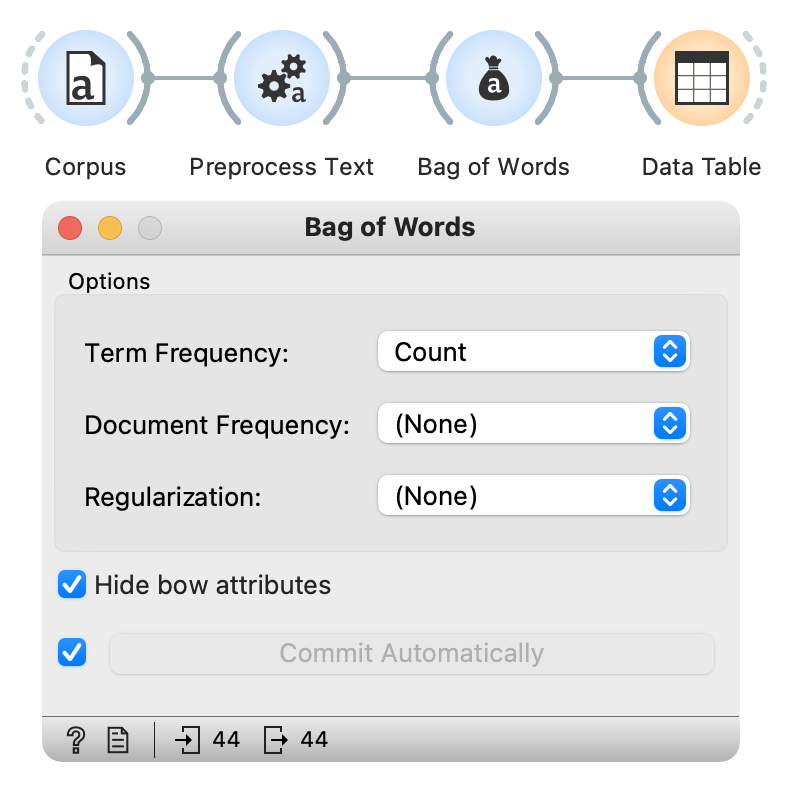
\includegraphics[width=\linewidth]{vreca-besed-workflow.png}
    \caption{}
\end{marginfigure}

Besede lahko preprosto preštejemo (TF ali term frequency) ali pa besede utežimo glede na to, kako pogosto se pojavijo v dokumentih (IDF ali inverse document frequency). S TF-IDF bodo pogoste besede imele nizko vrednost, saj se pojavijo velikokrat pri velikem deležu dokumentov, medtem ko bodo imele pomembne besede visoko vrednost, saj se pojavijo pogosto v majhnem deležu dokumentov.

Podatke pošilje v gradnik Bag of Words in od tam naprej v Data Table. Vidimo nov stolpec, ki vsebuje pojavitve besed za vsak dokument. Sedaj imamo številke in končno lahko pričnemo z analizo!

\begin{figure*}[h]
    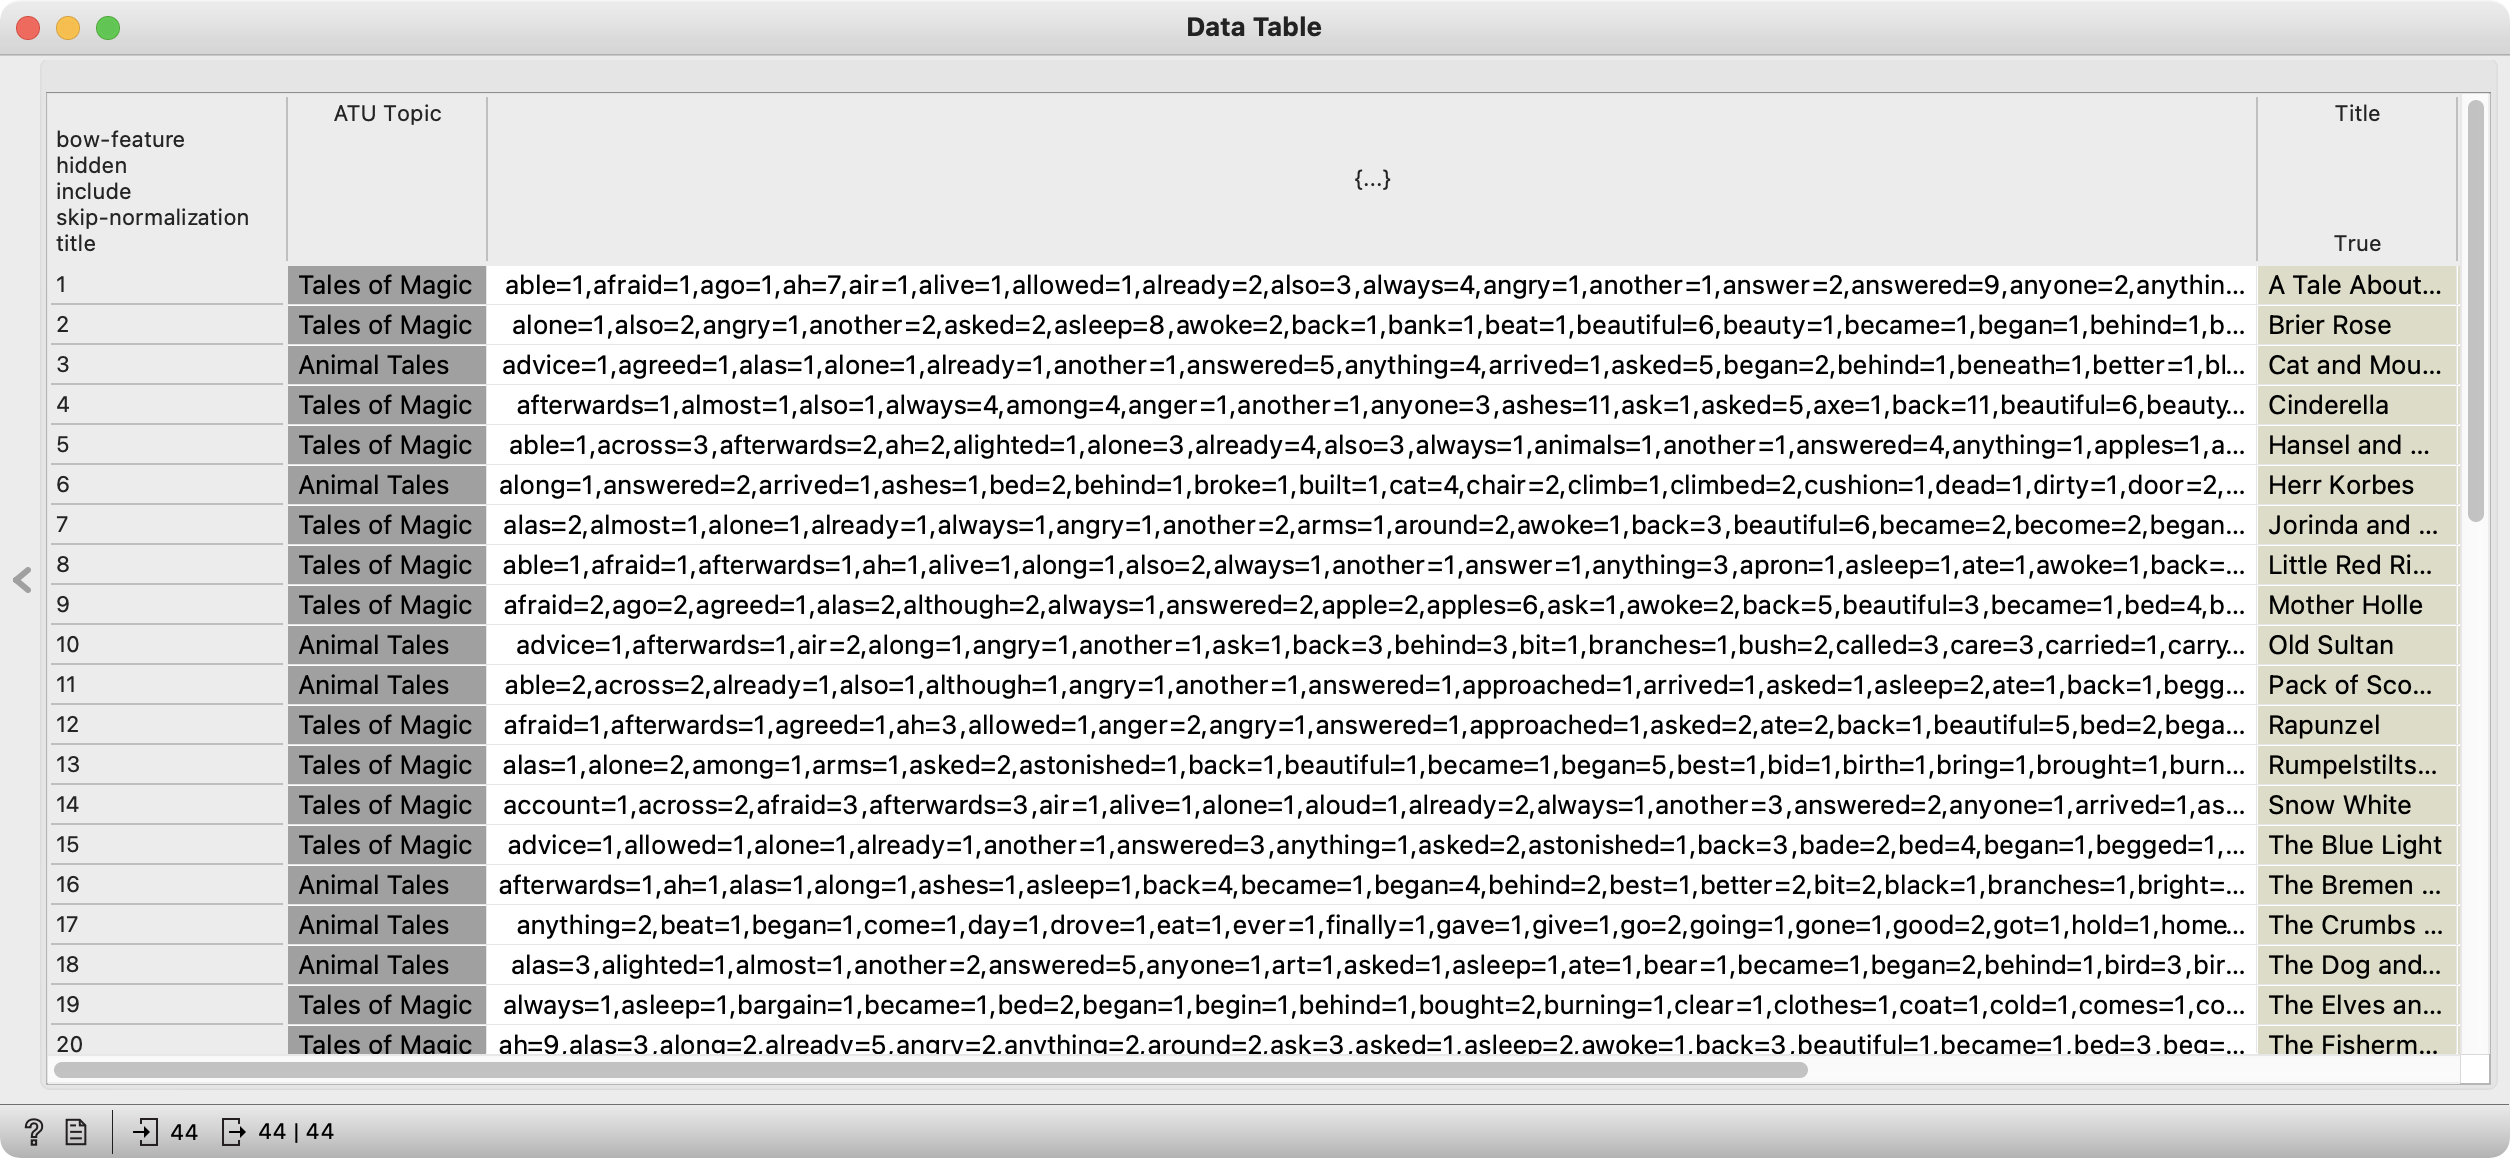
\includegraphics[width=\linewidth]{vreca-besed-table.png}%
    \caption{}
    \label{fig:004-vreca-besed-table}
  \end{figure*}
